\section{AC: Activity Clustering}
\label{sec:clustering:ac}

Initial clusters provided by $SA^3$ are expanded in this step, using context knowledge and time-based metrics for action aggregation. Assume Figure \ref{fig-initial-clusters} shows the output of $SA^3$ for a concrete sequence of actions. Dashes are time intervals without any action. Circles represent actions that are in one or more IAMs (two circles do not necessarily have to be the same action). Crosses are actions that are not included in any IAM. 

\begin{figure}[htbp]%[!t]
\centering
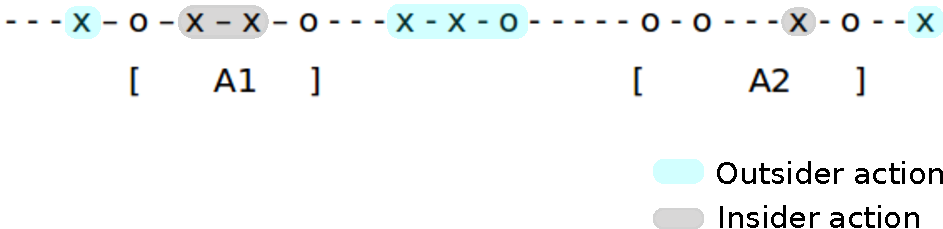
\includegraphics[width=\textwidth]{clustering_ex_complete.pdf}
    \caption{Output of $SA^3$ for a concrete sequence of actions.}
    \label{fig-initial-clusters}
\end{figure}

$SA^3$ detects activities $A_1$ and $A_2$ in that sequence of actions. That output has to be interpreted as the initialization of a clustering algorithm, so only actions that are in the IAM of the detected activity can be really considered part of that activity. Every action that is inside $A_1$ or $A_2$ but is not in their IAMs is considered an \textbf{insider}, while every action out of detected activities is an \textbf{outsider}.

Due to single-user single-activity scenario constraint, an insider may pertain to its wrapping activity or to none, i.e. it has been produced by noise. But an outsider can pertain to its previous activity, next activity or to none. This fact demands a different treatment for both cases. $AC$ first treats all insider actions and afterwards computes all outsiders using different approaches.

\textbf{Insiders:} to decide whether an insider has to be added to its wrapping activity, a compatibility function between an activity and an action is defined:

\begin{equation}
 Comp(A, a) = Loc(A, a) \wedge Type(A, a)
\end{equation}

\noindent where $A$ is an activity and $a$ is an action. $Loc(A, a)$ is the location compatibility between an activity and an action, defined as in Section \ref{subsec-sa3}. $Type(A, a)$ is the type compatibility between an activity and an action. It is calculated as the intersection between the list of types of the object which has been mapped to action $a$ and the type of the activity $A$. Type information for objects and activities is in the context knowledge. 

Hence an insider action $a$ will only be aggregated to its wrapping activity $A$, if $Comp(A, a) = True$, i.e. the insider has been executed in the same location of the activity, and its purpose is compatible with the activity type. 

\textbf{Outsiders:} as an outsider can be aggregated to its previous or next activity, first of all the algorithm checks the feasibility of both options, defining the \textit{candidate function}:

\begin{equation}
 Cand(A, a) = Comp(A, a) \wedge InRange(A, a)
\end{equation}

\noindent An activity $A$ is a candidate activity for action $a$, if they are compatible ($Comp(A, a) = True$) and in range ($InRange(A, a) = True$). $InRange$ function captures the time feasibility. For example, if an action has been executed two hours before an activity whose estimated duration is three minutes, it should not be aggregated to that activity. To capture time feasibility, the duration given by the expert in an IAM is interpreted as the standard deviation for concrete executions of that activity, i.e. the vast majority of the activities executed by any user, will lie inside the time area limited by the duration. This can be seen in Figure \ref{fig-in-range}. So time distances among actions pertaining to a concrete activity are modeled by a Gaussian distribution, where the duration estimation given by the expert for that activity is the standard deviation. A Gaussian distribution has been selected, because it captures perfectly the idea of activity duration as a time estimation where the majority of executions of that activity occur. The probability for actions of an activity to lie in the area limited by the duration estimation is very high and gets lower as it gets further from that duration.

Nevertheless, due to human behavior variations, there will be some executions whose duration is outside the standard deviation. To capture those executions, $InRange$ function considers all the actions lying inside two standard deviations. For a concrete activity execution, the mean of the activity is calculated as the center of the detected start and end of the activity, as given by $SA^3$. Hence, in the case depicted in Figure \ref{fig-in-range}, the outsider action is in range with activities $A_1$ and $A_2$. 

\begin{figure}[!t]
\centering
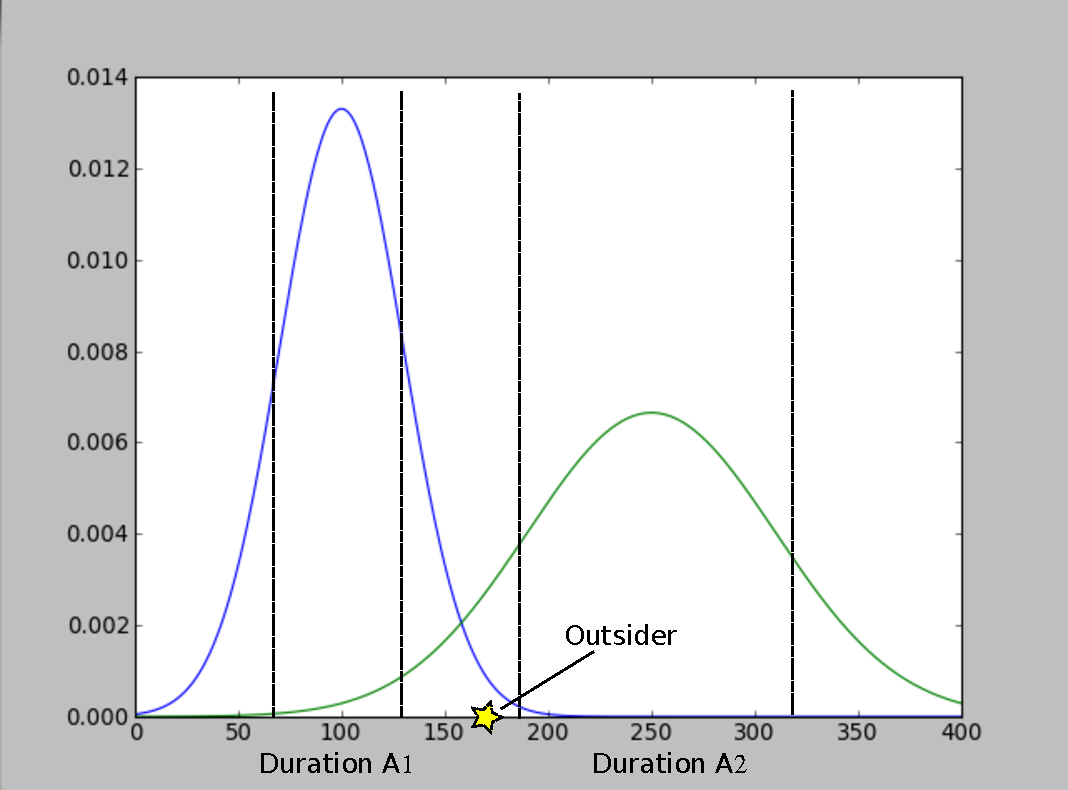
\includegraphics[width=\textwidth]{in_range_criterion.pdf}
    \caption{Gaussian distributions of activity durations for activities $A_1$ and $A_2$. Vertical lines show the standard deviation and the star represents an outsider action.}
    \label{fig-in-range}
\end{figure}

Using the candidate function, the following cases can be faced for an outsider action $a$ and surrounding activities $A_1$ and $A_2$:

\begin{enumerate}
 \item $Cand(A_1, a) = Cand(A_2, a) = False \rightarrow$ $a$ is noise
 \item $Cand(A_1, a) = True \wedge Cand(A_2, a) = False \rightarrow$ aggregate $a$ to $A_1$
 \item $Cand(A_1, a) = False \wedge Cand(A_2, a) = True \rightarrow$ aggregate $a$ to $A_2$
 \item $Cand(A_1, a) = Cand(A_2, a) = True \rightarrow$ need of a new heuristic
\end{enumerate}

For the fourth case, a new heuristic is defined which states that an outsider action $a$ will be aggregated to the time closest activity:

\begin{equation}
 min\{\Delta_t(A_1, a), \Delta_t(A_2, a)\}
\end{equation}

To implement this heuristic, a definition for $\Delta_t(A, a)$, the time distance between an activity and an action, is needed. As an activity has a duration and an action is described by a time instant, three time metrics are proposed:

\begin{enumerate}
 \item Simple time distance: the distance between the center of the activity as given by $SA^3$ and the action time coordinate.
 \begin{equation}
 \label{eq-t1}
  \Delta_t(A, a) = | C_A - t_a |,\ where \ C_A = \frac{t_{end} ^{SA^3} - t_{start} ^{SA^3}}{2}
 \end{equation}
 \item Normalized time distance: simple time distance normalized by the duration of the activity as given by the expert.
 \begin{equation}
 \label{eq-t2}
  \Delta_t(A, a) = \frac{| C_A - t_a |}{Duration_A} ,\ where \ C_A = \frac{t_{end} ^{SA^3} - t_{start} ^{SA^3}}{2}
 \end{equation}
 \item Dynamic center normalized time distance: only used for previous activity, it dynamically calculates the center of the activity depending on already aggregated actions.
 \begin{equation}
 \label{eq-t3}
  \Delta_t(A, a) = \frac{| C_A - t_a |}{Duration_A} ,\ where \ C_A = \frac{t_{start} ^{AC} + Duration_A}{2}
 \end{equation}
\end{enumerate}

Let us explain the third time distance. As outsiders are treated in time order for convenience, when treating outsider $a$, its previous activity's previous actions have already been treated. This means that the start of that previous activity has been fixed. In contrast with time metrics 1 and 2, where activity start and end were given by $SA^3$ and activity duration was assumed to be located symmetrically around the center of the activity, the third time metrics uses the start time of the previous activity as found by $AC$. Afterwards, the center of the activity is calculated projecting the duration from the starting point. This makes previous activity treatment more accurate. However, notice that the same cannot be applied to the next activity, since it has not been yet treated. Hence, the best guess is to keep using start and end times provided by $SA^3$.

To sum up, the $AC$ algorithm takes the results of $SA^3$. First, it treats insiders for all the activities detected by $SA^3$, using the compatibility function. Afterwards, it treats outsiders in time order, using the candidate function and defined three time metrics. The output of the algorithm is a labeled sensor activation dataset and a file where all activity clusters and their occurrence frequencies can be found. %Additionally, that file contains: (i) the frequency of each activity cluster, (ii) duration statistics (mean and standard deviation), (ii) frequencies of used objects and actions and (iii) frequencies of locations per activity. 